NeXus is an effort by an international group of scientists to define a common data exchange and archival format for neutron, X-ray and muon experiments. NeXus is built on top of the scientific data format HDF5 and adds domain-specific rules for organizing data within HDF5 files, in addition to a dictionary of well defined domain-specific field names. The NeXus data format has two purposes. First, it defines a format that can serve as a container for all relevant data associated with a beamline. This is a very important use case. Second, it defines standards in the form of application definitions for the exchange of data between applications. NeXus provides structures for raw experimental data as well as for processed data.

A recent addition to the NeXus standard means components that are used in experiments can specify shape definition to describe their placement, size and geometry. Transformations (NXtransformations) can be applied to these components when their position changes during or before the experiment. 

\begin{figure}
\caption{A typical nexus file layout with shape definition}
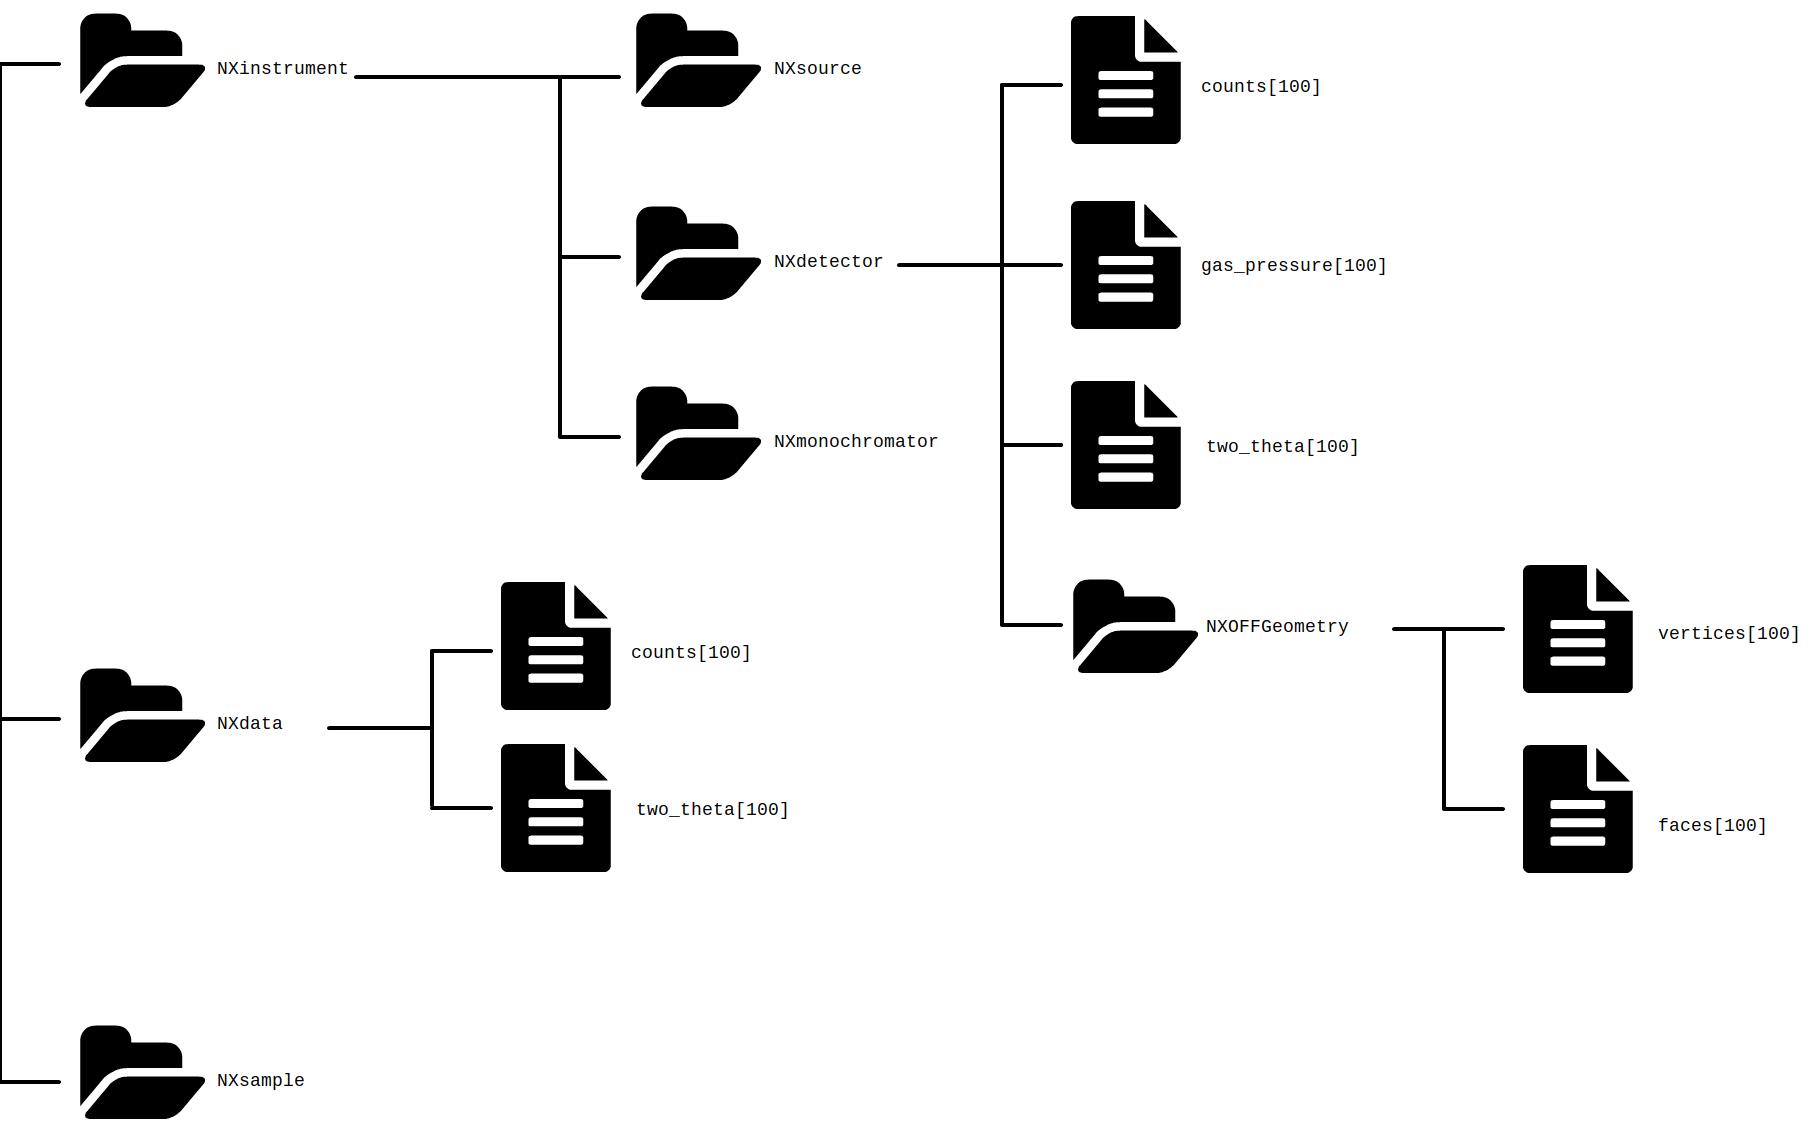
\includegraphics[width=\linewidth]{nexusdiagram.png}
\end{figure}

Currently, there is no tool for visualising and editing NeXus files. The section below describes our solution for this and how we are implementing a tool containing this functionality. NeXus files are outputted by the experiment, and tools need to be configured to write them. This is currently being done manually by editing large JSON files which is both fragile and time-consuming.
